\section{Background}
\textbf{\textit{present contextual or prerequisite information that is important or essential to understand the main body of the thesis}}

Arbetssätt \& flöde

Competitors


The process of creating a web-application is typically done in three major steps: 
\begin{itemize}
  \item Design
  \item Develop
  \item Publish
\end{itemize}

The tool that this project is creating is will almost follow these three steps except the last one. Instead of publishing however the components that will be generated need to be distributed between designer and developer. Therefor \textbf{\textit{publish}}, for this project is replaced by \textbf{\textit{distribute}}.

All these steps are often, if not always, done iteratively within them selfs and as a whole cycle. However there must be some sort of design to start a meaningful and useful development effort. If there is nothing that has been developed there is nothing to publish. So therefore these three must be done in order. 

The tool that this project produced has a part in all these three steps.\\ 
Design(Figma) --\textgreater Develop(Figma API, FigmaConverter) --\textgreater Distribute(package manager (NPM)).\\
In this section we will dive deeper in how to traverse these steps, and how it is possible to automate it.


\begin{figure}[H]
  \centering
  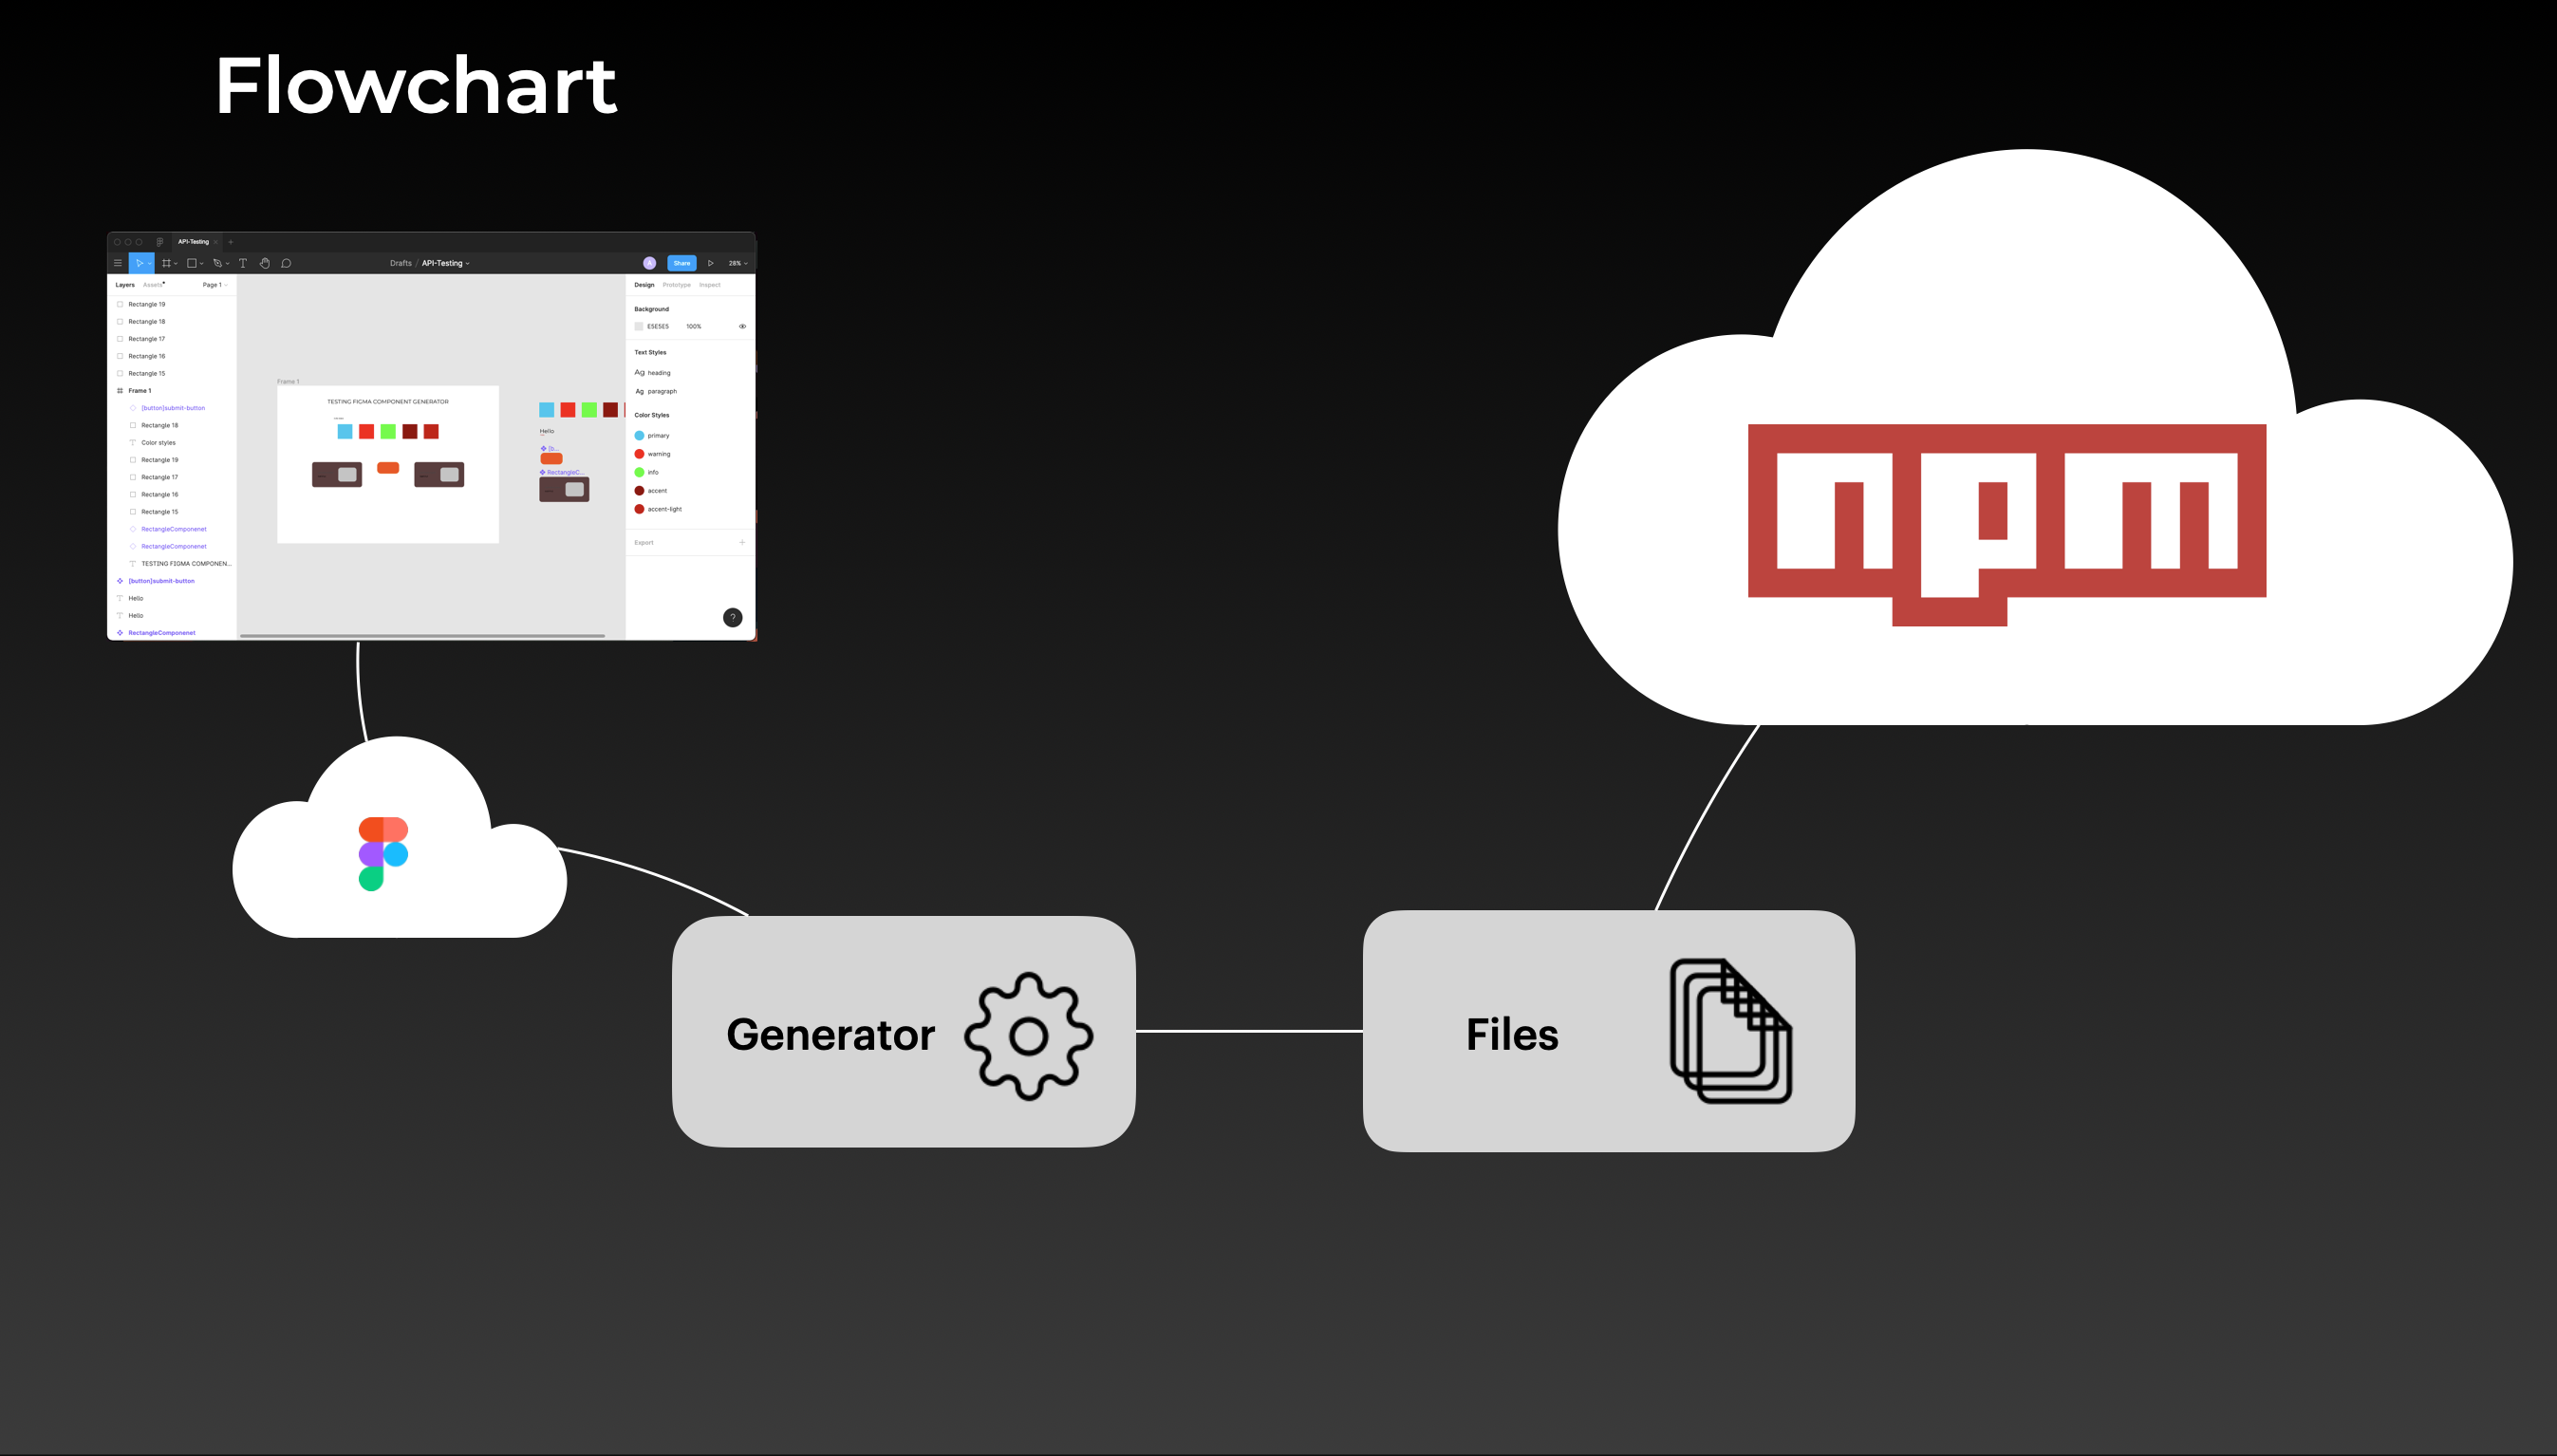
\includegraphics[width=0.8\linewidth]{images/flow.png}
  \caption{Chart over how data flows in the program}%
  \label{fig:flow}
\end{figure}

\subsection{Competitors}%
\label{sub:Competitors}
The idea of making a design program generate functional code is not new. In this section some of the competitors of this genre of programs will be brought up and compared.

\subsubsection{Webflow}
Webflow was founded in 2013 and is a product from the famous program Y Combinator. Webflow allows the user to design, create and publish a website all from their program. Webflow is, as Figma, a network based application that works form a web browser. 


Webflows website: \cite{ResponsiveWebDesign} 

\subsubsection{Visly}%
\label{ssub:Visly}
Visly website: \cite{vislyVisly} 
Visly is was founded in 2018 and is very similar to Figma in how the user designs the product. Visly uses the design to create React components \cite{facebookincReactJavaScriptLibrary}. React is a component based JavaScript framework made by Facebook. Visly essentially makes it possible to create these components visually.

\subsubsection{Bravo}%
\label{ssub:Bravo}

Build Native IOS och Android apps with Figma. Think this can be the closest to the what I'm trying to do. 

\subsubsection{Comparison}%
\label{ssub:Comparison}




